\documentclass[1p]{elsarticle_modified}
%\bibliographystyle{elsarticle-num}

%\usepackage[colorlinks]{hyperref}
%\usepackage{abbrmath_seonhwa} %\Abb, \Ascr, \Acal ,\Abf, \Afrak
\usepackage{amsfonts}
\usepackage{amssymb}
\usepackage{amsmath}
\usepackage{amsthm}
\usepackage{scalefnt}
\usepackage{amsbsy}
\usepackage{kotex}
\usepackage{caption}
\usepackage{subfig}
\usepackage{color}
\usepackage{graphicx}
\usepackage{xcolor} %% white, black, red, green, blue, cyan, magenta, yellow
\usepackage{float}
\usepackage{setspace}
\usepackage{hyperref}

\usepackage{tikz}
\usetikzlibrary{arrows}

\usepackage{multirow}
\usepackage{array} % fixed length table
\usepackage{hhline}

%%%%%%%%%%%%%%%%%%%%%
\makeatletter
\renewcommand*\env@matrix[1][\arraystretch]{%
	\edef\arraystretch{#1}%
	\hskip -\arraycolsep
	\let\@ifnextchar\new@ifnextchar
	\array{*\c@MaxMatrixCols c}}
\makeatother %https://tex.stackexchange.com/questions/14071/how-can-i-increase-the-line-spacing-in-a-matrix
%%%%%%%%%%%%%%%

\usepackage[normalem]{ulem}

\newcommand{\msout}[1]{\ifmmode\text{\sout{\ensuremath{#1}}}\else\sout{#1}\fi}
%SOURCE: \msout is \stkout macro in https://tex.stackexchange.com/questions/20609/strikeout-in-math-mode

\newcommand{\cancel}[1]{
	\ifmmode
	{\color{red}\msout{#1}}
	\else
	{\color{red}\sout{#1}}
	\fi
}

\newcommand{\add}[1]{
	{\color{blue}\uwave{#1}}
}

\newcommand{\replace}[2]{
	\ifmmode
	{\color{red}\msout{#1}}{\color{blue}\uwave{#2}}
	\else
	{\color{red}\sout{#1}}{\color{blue}\uwave{#2}}
	\fi
}

\newcommand{\Sol}{\mathcal{S}} %segment
\newcommand{\D}{D} %diagram
\newcommand{\A}{\mathcal{A}} %arc


%%%%%%%%%%%%%%%%%%%%%%%%%%%%%5 test

\def\sl{\operatorname{\textup{SL}}(2,\Cbb)}
\def\psl{\operatorname{\textup{PSL}}(2,\Cbb)}
\def\quan{\mkern 1mu \triangleright \mkern 1mu}

\theoremstyle{definition}
\newtheorem{thm}{Theorem}[section]
\newtheorem{prop}[thm]{Proposition}
\newtheorem{lem}[thm]{Lemma}
\newtheorem{ques}[thm]{Question}
\newtheorem{cor}[thm]{Corollary}
\newtheorem{defn}[thm]{Definition}
\newtheorem{exam}[thm]{Example}
\newtheorem{rmk}[thm]{Remark}
\newtheorem{alg}[thm]{Algorithm}

\newcommand{\I}{\sqrt{-1}}
\begin{document}

%\begin{frontmatter}
%
%\title{Boundary parabolic representations of knots up to 8 crossings}
%
%%% Group authors per affiliation:
%\author{Yunhi Cho} 
%\address{Department of Mathematics, University of Seoul, Seoul, Korea}
%\ead{yhcho@uos.ac.kr}
%
%
%\author{Seonhwa Kim} %\fnref{s_kim}}
%\address{Center for Geometry and Physics, Institute for Basic Science, Pohang, 37673, Korea}
%\ead{ryeona17@ibs.re.kr}
%
%\author{Hyuk Kim}
%\address{Department of Mathematical Sciences, Seoul National University, Seoul 08826, Korea}
%\ead{hyukkim@snu.ac.kr}
%
%\author{Seokbeom Yoon}
%\address{Department of Mathematical Sciences, Seoul National University, Seoul, 08826,  Korea}
%\ead{sbyoon15@snu.ac.kr}
%
%\begin{abstract}
%We find all boundary parabolic representation of knots up to 8 crossings.
%
%\end{abstract}
%\begin{keyword}
%    \MSC[2010] 57M25 
%\end{keyword}
%
%\end{frontmatter}

%\linenumbers
%\tableofcontents
%
\newcommand\colored[1]{\textcolor{white}{\rule[-0.35ex]{0.8em}{1.4ex}}\kern-0.8em\color{red} #1}%
%\newcommand\colored[1]{\textcolor{white}{ #1}\kern-2.17ex	\textcolor{white}{ #1}\kern-1.81ex	\textcolor{white}{ #1}\kern-2.15ex\color{red}#1	}

{\Large $\underline{12a_{0236}~(K12a_{0236})}$}

\setlength{\tabcolsep}{10pt}
\renewcommand{\arraystretch}{1.6}
\vspace{1cm}\begin{tabular}{m{100pt}>{\centering\arraybackslash}m{274pt}}
\multirow{5}{120pt}{
	\centering
	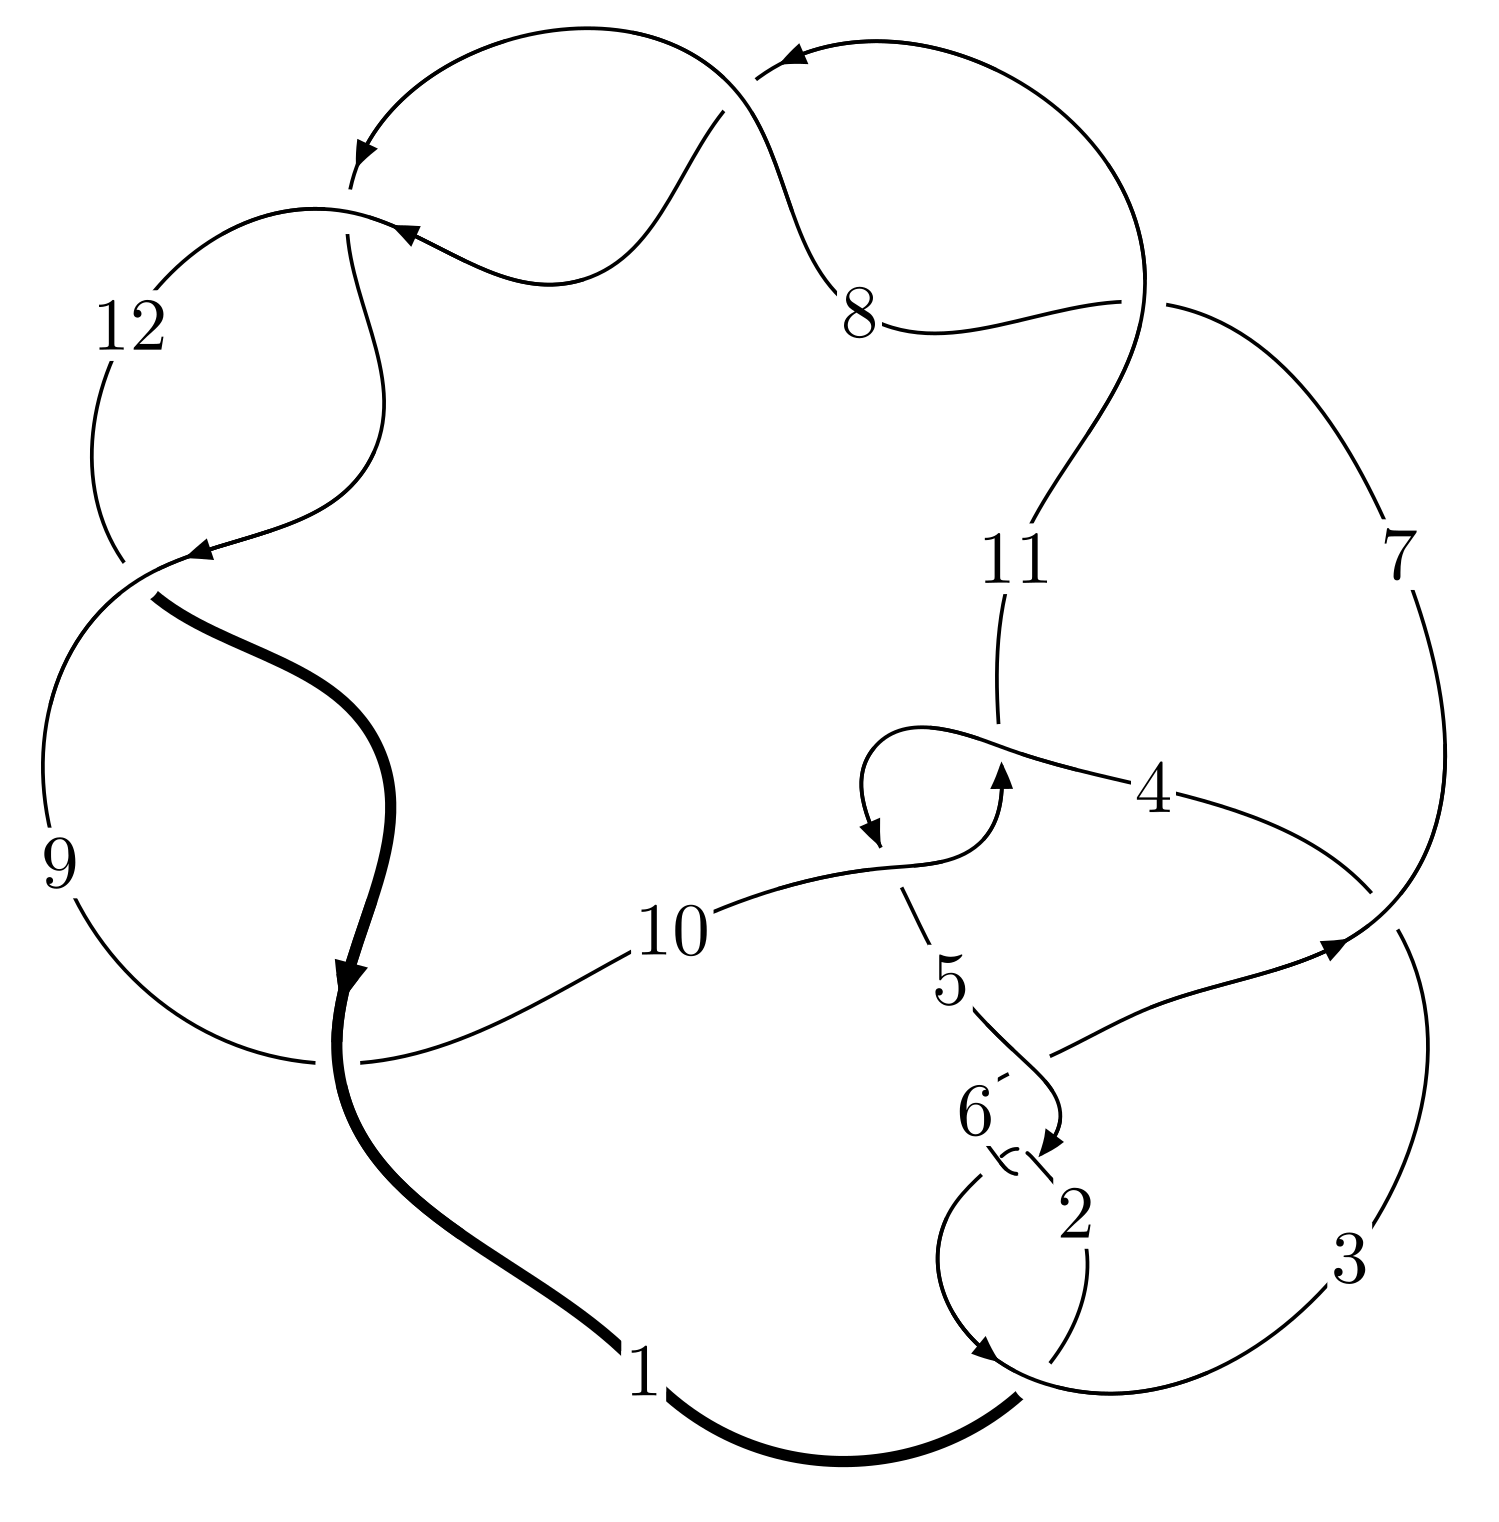
\includegraphics[width=112pt]{../../../GIT/diagram.site/Diagrams/png/1037_12a_0236.png}\\
\ \ \ A knot diagram\footnotemark}&
\allowdisplaybreaks
\textbf{Linearized knot diagam} \\
\cline{2-2}
 &
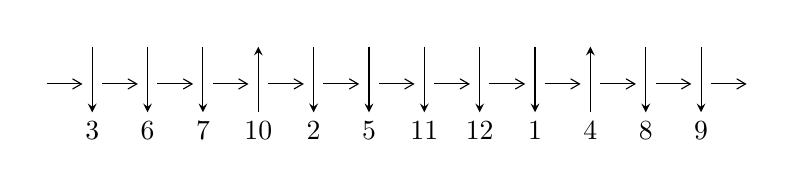
\begin{tikzpicture}[x=20pt, y=17pt]
	% nodes
	\node (C0) at (0, 0) {};
	\node (C1) at (1, 0) {};
	\node (C1U) at (1, +1) {};
	\node (C1D) at (1, -1) {3};

	\node (C2) at (2, 0) {};
	\node (C2U) at (2, +1) {};
	\node (C2D) at (2, -1) {6};

	\node (C3) at (3, 0) {};
	\node (C3U) at (3, +1) {};
	\node (C3D) at (3, -1) {7};

	\node (C4) at (4, 0) {};
	\node (C4U) at (4, +1) {};
	\node (C4D) at (4, -1) {10};

	\node (C5) at (5, 0) {};
	\node (C5U) at (5, +1) {};
	\node (C5D) at (5, -1) {2};

	\node (C6) at (6, 0) {};
	\node (C6U) at (6, +1) {};
	\node (C6D) at (6, -1) {5};

	\node (C7) at (7, 0) {};
	\node (C7U) at (7, +1) {};
	\node (C7D) at (7, -1) {11};

	\node (C8) at (8, 0) {};
	\node (C8U) at (8, +1) {};
	\node (C8D) at (8, -1) {12};

	\node (C9) at (9, 0) {};
	\node (C9U) at (9, +1) {};
	\node (C9D) at (9, -1) {1};

	\node (C10) at (10, 0) {};
	\node (C10U) at (10, +1) {};
	\node (C10D) at (10, -1) {4};

	\node (C11) at (11, 0) {};
	\node (C11U) at (11, +1) {};
	\node (C11D) at (11, -1) {8};

	\node (C12) at (12, 0) {};
	\node (C12U) at (12, +1) {};
	\node (C12D) at (12, -1) {9};
	\node (C13) at (13, 0) {};

	% arrows
	\draw[->,>={angle 60}]
	(C0) edge (C1) (C1) edge (C2) (C2) edge (C3) (C3) edge (C4) (C4) edge (C5) (C5) edge (C6) (C6) edge (C7) (C7) edge (C8) (C8) edge (C9) (C9) edge (C10) (C10) edge (C11) (C11) edge (C12) (C12) edge (C13) ;	\draw[->,>=stealth]
	(C1U) edge (C1D) (C2U) edge (C2D) (C3U) edge (C3D) (C4D) edge (C4U) (C5U) edge (C5D) (C6U) edge (C6D) (C7U) edge (C7D) (C8U) edge (C8D) (C9U) edge (C9D) (C10D) edge (C10U) (C11U) edge (C11D) (C12U) edge (C12D) ;
	\end{tikzpicture} \\
\hhline{~~} \\& 
\textbf{Solving Sequence} \\ \cline{2-2} 
 &
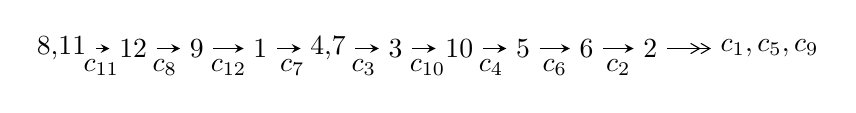
\begin{tikzpicture}[x=23pt, y=7pt]
	% node
	\node (A0) at (-1/8, 0) {8,11};
	\node (A1) at (1, 0) {12};
	\node (A2) at (2, 0) {9};
	\node (A3) at (3, 0) {1};
	\node (A4) at (65/16, 0) {4,7};
	\node (A5) at (41/8, 0) {3};
	\node (A6) at (49/8, 0) {10};
	\node (A7) at (57/8, 0) {5};
	\node (A8) at (65/8, 0) {6};
	\node (A9) at (73/8, 0) {2};
	\node (C1) at (1/2, -1) {$c_{11}$};
	\node (C2) at (3/2, -1) {$c_{8}$};
	\node (C3) at (5/2, -1) {$c_{12}$};
	\node (C4) at (7/2, -1) {$c_{7}$};
	\node (C5) at (37/8, -1) {$c_{3}$};
	\node (C6) at (45/8, -1) {$c_{10}$};
	\node (C7) at (53/8, -1) {$c_{4}$};
	\node (C8) at (61/8, -1) {$c_{6}$};
	\node (C9) at (69/8, -1) {$c_{2}$};
	\node (A10) at (11, 0) {$c_{1},c_{5},c_{9}$};

	% edge
	\draw[->,>=stealth]	
	(A0) edge (A1) (A1) edge (A2) (A2) edge (A3) (A3) edge (A4) (A4) edge (A5) (A5) edge (A6) (A6) edge (A7) (A7) edge (A8) (A8) edge (A9) ;
	\draw[->>,>={angle 60}]	
	(A9) edge (A10);
\end{tikzpicture} \\ 

\end{tabular} \\

\footnotetext{
The image of knot diagram is generated by the software ``\textbf{Draw programme}" developed by Andrew Bartholomew(\url{http://www.layer8.co.uk/maths/draw/index.htm\#Running-draw}), where we modified some parts for our purpose(\url{https://github.com/CATsTAILs/LinksPainter}).
}\phantom \\ \newline 
\centering \textbf{Ideals for irreducible components\footnotemark of $X_{\text{par}}$} 
 
\begin{align*}
I^u_{1}&=\langle 
15 u^{53}+20 u^{52}+\cdots+2 b-8,\;49 u^{53}+76 u^{52}+\cdots+4 a-12,\;u^{54}+3 u^{53}+\cdots+3 u-1\rangle \\
I^u_{2}&=\langle 
b,\;a^3- a^2 u+a^2-2 a u+4 a-2 u+3,\;u^2- u-1\rangle \\
I^u_{3}&=\langle 
b+1,\;a,\;u+1\rangle \\
\\
\end{align*}
\raggedright * 3 irreducible components of $\dim_{\mathbb{C}}=0$, with total 61 representations.\\
\footnotetext{All coefficients of polynomials are rational numbers. But the coefficients are sometimes approximated in decimal forms when there is not enough margin.}
\newpage
\renewcommand{\arraystretch}{1}
\centering \section*{I. $I^u_{1}= \langle 15 u^{53}+20 u^{52}+\cdots+2 b-8,\;49 u^{53}+76 u^{52}+\cdots+4 a-12,\;u^{54}+3 u^{53}+\cdots+3 u-1 \rangle$}
\flushleft \textbf{(i) Arc colorings}\\
\begin{tabular}{m{7pt} m{180pt} m{7pt} m{180pt} }
\flushright $a_{8}=$&$\begin{pmatrix}0\\u\end{pmatrix}$ \\
\flushright $a_{11}=$&$\begin{pmatrix}1\\0\end{pmatrix}$ \\
\flushright $a_{12}=$&$\begin{pmatrix}1\\u^2\end{pmatrix}$ \\
\flushright $a_{9}=$&$\begin{pmatrix}- u\\- u^3+u\end{pmatrix}$ \\
\flushright $a_{1}=$&$\begin{pmatrix}- u^2+1\\- u^4+2 u^2\end{pmatrix}$ \\
\flushright $a_{4}=$&$\begin{pmatrix}-\frac{49}{4} u^{53}-19 u^{52}+\cdots-\frac{105}{4} u+3\\-\frac{15}{2} u^{53}-10 u^{52}+\cdots-\frac{27}{2} u+4\end{pmatrix}$ \\
\flushright $a_{7}=$&$\begin{pmatrix}u\\u\end{pmatrix}$ \\
\flushright $a_{3}=$&$\begin{pmatrix}-\frac{7}{4} u^{53}-\frac{17}{4} u^{52}+\cdots-\frac{23}{4} u-\frac{9}{4}\\3 u^{53}+\frac{19}{4} u^{52}+\cdots+7 u-\frac{5}{4}\end{pmatrix}$ \\
\flushright $a_{10}=$&$\begin{pmatrix}u^3-2 u\\u^5-3 u^3+u\end{pmatrix}$ \\
\flushright $a_{5}=$&$\begin{pmatrix}\frac{9}{4} u^{53}-\frac{327}{4} u^{51}+\cdots+\frac{9}{4} u-5\\\frac{19}{2} u^{53}+12 u^{52}+\cdots+\frac{39}{2} u-5\end{pmatrix}$ \\
\flushright $a_{6}=$&$\begin{pmatrix}\frac{1}{4} u^{53}+\frac{3}{4} u^{52}+\cdots+\frac{23}{4} u+\frac{5}{4}\\- u^{16}+10 u^{14}+\cdots-6 u^3-4 u^2\end{pmatrix}$ \\
\flushright $a_{2}=$&$\begin{pmatrix}-\frac{1}{4} u^{52}-\frac{1}{2} u^{51}+\cdots-\frac{9}{2} u-\frac{1}{4}\\\frac{1}{4} u^{53}+\frac{1}{2} u^{52}+\cdots+\frac{11}{2} u^2+\frac{5}{4} u\end{pmatrix}$\\&\end{tabular}
\flushleft \textbf{(ii) Obstruction class $= -1$}\\~\\
\flushleft \textbf{(iii) Cusp Shapes $= -8 u^{53}-6 u^{52}+\cdots-19 u+\frac{1}{2}$}\\~\\
\newpage\renewcommand{\arraystretch}{1}
\flushleft \textbf{(iv) u-Polynomials at the component}\newline \\
\begin{tabular}{m{50pt}|m{274pt}}
Crossings & \hspace{64pt}u-Polynomials at each crossing \\
\hline $$\begin{aligned}c_{1},c_{6}\end{aligned}$$&$\begin{aligned}
&u^{54}+18 u^{53}+\cdots+28 u+1
\end{aligned}$\\
\hline $$\begin{aligned}c_{2},c_{5}\end{aligned}$$&$\begin{aligned}
&u^{54}+2 u^{53}+\cdots-14 u^2+1
\end{aligned}$\\
\hline $$\begin{aligned}c_{3}\end{aligned}$$&$\begin{aligned}
&u^{54}-4 u^{53}+\cdots-2672 u+433
\end{aligned}$\\
\hline $$\begin{aligned}c_{4},c_{10}\end{aligned}$$&$\begin{aligned}
&u^{54}+2 u^{53}+\cdots-224 u-64
\end{aligned}$\\
\hline $$\begin{aligned}c_{7},c_{8},c_{9}\\c_{11},c_{12}\end{aligned}$$&$\begin{aligned}
&u^{54}+3 u^{53}+\cdots+3 u-1
\end{aligned}$\\
\hline
\end{tabular}\\~\\
\newpage\renewcommand{\arraystretch}{1}
\flushleft \textbf{(v) Riley Polynomials at the component}\newline \\
\begin{tabular}{m{50pt}|m{274pt}}
Crossings & \hspace{64pt}Riley Polynomials at each crossing \\
\hline $$\begin{aligned}c_{1},c_{6}\end{aligned}$$&$\begin{aligned}
&y^{54}+38 y^{53}+\cdots-252 y+1
\end{aligned}$\\
\hline $$\begin{aligned}c_{2},c_{5}\end{aligned}$$&$\begin{aligned}
&y^{54}-18 y^{53}+\cdots-28 y+1
\end{aligned}$\\
\hline $$\begin{aligned}c_{3}\end{aligned}$$&$\begin{aligned}
&y^{54}-22 y^{53}+\cdots-7170760 y+187489
\end{aligned}$\\
\hline $$\begin{aligned}c_{4},c_{10}\end{aligned}$$&$\begin{aligned}
&y^{54}+36 y^{53}+\cdots-1024 y+4096
\end{aligned}$\\
\hline $$\begin{aligned}c_{7},c_{8},c_{9}\\c_{11},c_{12}\end{aligned}$$&$\begin{aligned}
&y^{54}-73 y^{53}+\cdots-33 y+1
\end{aligned}$\\
\hline
\end{tabular}\\~\\
\newpage\flushleft \textbf{(vi) Complex Volumes and Cusp Shapes}
$$\begin{array}{c|c|c}  
\text{Solutions to }I^u_{1}& \I (\text{vol} + \sqrt{-1}CS) & \text{Cusp shape}\\
 \hline 
\begin{aligned}
u &= -0.996240 + 0.174836 I \\
a &= -0.046917 - 0.171089 I \\
b &= -1.041700 + 0.270047 I\end{aligned}
 & -0.93612 + 5.33064 I & \phantom{-0.000000 } 0 \\ \hline\begin{aligned}
u &= -0.996240 - 0.174836 I \\
a &= -0.046917 + 0.171089 I \\
b &= -1.041700 - 0.270047 I\end{aligned}
 & -0.93612 - 5.33064 I & \phantom{-0.000000 } 0 \\ \hline\begin{aligned}
u &= -0.921952 + 0.190975 I \\
a &= \phantom{-}0.120199 + 0.149841 I \\
b &= \phantom{-}0.923078 - 0.334826 I\end{aligned}
 & -0.122335 + 0.095210 I & -8.00000 + 0. I\phantom{ +0.000000I} \\ \hline\begin{aligned}
u &= -0.921952 - 0.190975 I \\
a &= \phantom{-}0.120199 - 0.149841 I \\
b &= \phantom{-}0.923078 + 0.334826 I\end{aligned}
 & -0.122335 - 0.095210 I & -8.00000 + 0. I\phantom{ +0.000000I} \\ \hline\begin{aligned}
u &= \phantom{-}1.064210 + 0.209793 I \\
a &= -0.63295 - 1.61348 I \\
b &= \phantom{-}0.282300 - 1.168280 I\end{aligned}
 & -4.75278 - 2.80286 I & \phantom{-0.000000 } 0 \\ \hline\begin{aligned}
u &= \phantom{-}1.064210 - 0.209793 I \\
a &= -0.63295 + 1.61348 I \\
b &= \phantom{-}0.282300 + 1.168280 I\end{aligned}
 & -4.75278 + 2.80286 I & \phantom{-0.000000 } 0 \\ \hline\begin{aligned}
u &= \phantom{-}1.030910 + 0.348284 I \\
a &= -0.95535 - 1.48256 I \\
b &= \phantom{-}0.541961 - 1.230030 I\end{aligned}
 & -3.03671 - 5.51505 I & \phantom{-0.000000 } 0 \\ \hline\begin{aligned}
u &= \phantom{-}1.030910 - 0.348284 I \\
a &= -0.95535 + 1.48256 I \\
b &= \phantom{-}0.541961 + 1.230030 I\end{aligned}
 & -3.03671 + 5.51505 I & \phantom{-0.000000 } 0 \\ \hline\begin{aligned}
u &= \phantom{-}1.050340 + 0.376575 I \\
a &= \phantom{-}0.96873 + 1.41375 I \\
b &= -0.57619 + 1.29485 I\end{aligned}
 & -4.25463 - 11.21320 I & \phantom{-0.000000 } 0 \\ \hline\begin{aligned}
u &= \phantom{-}1.050340 - 0.376575 I \\
a &= \phantom{-}0.96873 - 1.41375 I \\
b &= -0.57619 - 1.29485 I\end{aligned}
 & -4.25463 + 11.21320 I & \phantom{-0.000000 } 0\\
 \hline 
 \end{array}$$\newpage$$\begin{array}{c|c|c}  
\text{Solutions to }I^u_{1}& \I (\text{vol} + \sqrt{-1}CS) & \text{Cusp shape}\\
 \hline 
\begin{aligned}
u &= \phantom{-}0.851855 + 0.026742 I \\
a &= -0.20081 - 2.78618 I \\
b &= \phantom{-}0.052036 - 0.745442 I\end{aligned}
 & \phantom{-}1.33981 - 2.97841 I & -16.2532 + 3.7844 I \\ \hline\begin{aligned}
u &= \phantom{-}0.851855 - 0.026742 I \\
a &= -0.20081 + 2.78618 I \\
b &= \phantom{-}0.052036 + 0.745442 I\end{aligned}
 & \phantom{-}1.33981 + 2.97841 I & -16.2532 - 3.7844 I \\ \hline\begin{aligned}
u &= \phantom{-}1.113960 + 0.306274 I \\
a &= \phantom{-}0.77810 + 1.39695 I \\
b &= -0.384474 + 1.331420 I\end{aligned}
 & -9.35844 - 4.90130 I & \phantom{-0.000000 } 0 \\ \hline\begin{aligned}
u &= \phantom{-}1.113960 - 0.306274 I \\
a &= \phantom{-}0.77810 - 1.39695 I \\
b &= -0.384474 - 1.331420 I\end{aligned}
 & -9.35844 + 4.90130 I & \phantom{-0.000000 } 0 \\ \hline\begin{aligned}
u &= \phantom{-}1.175560 + 0.167588 I \\
a &= \phantom{-}0.43398 + 1.38174 I \\
b &= -0.143925 + 1.276040 I\end{aligned}
 & -6.63511 + 1.61390 I & \phantom{-0.000000 } 0 \\ \hline\begin{aligned}
u &= \phantom{-}1.175560 - 0.167588 I \\
a &= \phantom{-}0.43398 - 1.38174 I \\
b &= -0.143925 - 1.276040 I\end{aligned}
 & -6.63511 - 1.61390 I & \phantom{-0.000000 } 0 \\ \hline\begin{aligned}
u &= -0.519490 + 0.531321 I \\
a &= -0.713490 - 0.165731 I \\
b &= -0.208766 + 1.145180 I\end{aligned}
 & -1.05139 - 3.92853 I & -12.01559 + 2.10078 I \\ \hline\begin{aligned}
u &= -0.519490 - 0.531321 I \\
a &= -0.713490 + 0.165731 I \\
b &= -0.208766 - 1.145180 I\end{aligned}
 & -1.05139 + 3.92853 I & -12.01559 - 2.10078 I \\ \hline\begin{aligned}
u &= -0.723166\phantom{ +0.000000I} \\
a &= \phantom{-}0.147422\phantom{ +0.000000I} \\
b &= \phantom{-}0.462202\phantom{ +0.000000I}\end{aligned}
 & -1.27288\phantom{ +0.000000I} & -6.75210\phantom{ +0.000000I} \\ \hline\begin{aligned}
u &= -0.542660 + 0.430784 I \\
a &= \phantom{-}0.615074 + 0.066547 I \\
b &= \phantom{-}0.268273 - 0.941014 I\end{aligned}
 & -0.103530 + 1.138840 I & -10.54250 - 3.54234 I\\
 \hline 
 \end{array}$$\newpage$$\begin{array}{c|c|c}  
\text{Solutions to }I^u_{1}& \I (\text{vol} + \sqrt{-1}CS) & \text{Cusp shape}\\
 \hline 
\begin{aligned}
u &= -0.542660 - 0.430784 I \\
a &= \phantom{-}0.615074 - 0.066547 I \\
b &= \phantom{-}0.268273 + 0.941014 I\end{aligned}
 & -0.103530 - 1.138840 I & -10.54250 + 3.54234 I \\ \hline\begin{aligned}
u &= -0.364228 + 0.577449 I \\
a &= -0.934188 - 0.148020 I \\
b &= \phantom{-}0.138461 + 1.174430 I\end{aligned}
 & -4.71225 + 1.89294 I & -15.7177 - 3.8918 I \\ \hline\begin{aligned}
u &= -0.364228 - 0.577449 I \\
a &= -0.934188 + 0.148020 I \\
b &= \phantom{-}0.138461 - 1.174430 I\end{aligned}
 & -4.71225 - 1.89294 I & -15.7177 + 3.8918 I \\ \hline\begin{aligned}
u &= -0.250036 + 0.633419 I \\
a &= -1.104300 - 0.206805 I \\
b &= \phantom{-}0.417478 + 1.191560 I\end{aligned}
 & -0.22294 + 7.78581 I & -9.62304 - 7.92359 I \\ \hline\begin{aligned}
u &= -0.250036 - 0.633419 I \\
a &= -1.104300 + 0.206805 I \\
b &= \phantom{-}0.417478 - 1.191560 I\end{aligned}
 & -0.22294 - 7.78581 I & -9.62304 + 7.92359 I \\ \hline\begin{aligned}
u &= -0.225695 + 0.589084 I \\
a &= \phantom{-}1.140710 + 0.141782 I \\
b &= -0.419400 - 1.081010 I\end{aligned}
 & \phantom{-}0.86035 + 2.32908 I & -7.32309 - 3.24267 I \\ \hline\begin{aligned}
u &= -0.225695 - 0.589084 I \\
a &= \phantom{-}1.140710 - 0.141782 I \\
b &= -0.419400 + 1.081010 I\end{aligned}
 & \phantom{-}0.86035 - 2.32908 I & -7.32309 + 3.24267 I \\ \hline\begin{aligned}
u &= \phantom{-}1.55391 + 0.02757 I \\
a &= -0.098217 - 0.452334 I \\
b &= -0.140479 - 0.824642 I\end{aligned}
 & -6.99883 - 2.48049 I & \phantom{-0.000000 } 0 \\ \hline\begin{aligned}
u &= \phantom{-}1.55391 - 0.02757 I \\
a &= -0.098217 + 0.452334 I \\
b &= -0.140479 + 0.824642 I\end{aligned}
 & -6.99883 + 2.48049 I & \phantom{-0.000000 } 0 \\ \hline\begin{aligned}
u &= -0.281495 + 0.312842 I \\
a &= \phantom{-}0.916828 - 0.383169 I \\
b &= -0.123921 - 0.686515 I\end{aligned}
 & -0.459739 + 0.937129 I & -7.88969 - 7.07124 I\\
 \hline 
 \end{array}$$\newpage$$\begin{array}{c|c|c}  
\text{Solutions to }I^u_{1}& \I (\text{vol} + \sqrt{-1}CS) & \text{Cusp shape}\\
 \hline 
\begin{aligned}
u &= -0.281495 - 0.312842 I \\
a &= \phantom{-}0.916828 + 0.383169 I \\
b &= -0.123921 + 0.686515 I\end{aligned}
 & -0.459739 - 0.937129 I & -7.88969 + 7.07124 I \\ \hline\begin{aligned}
u &= \phantom{-}0.135244 + 0.362504 I \\
a &= \phantom{-}2.08092 + 0.05555 I \\
b &= -0.644171 - 0.344545 I\end{aligned}
 & \phantom{-}3.08884 + 1.84557 I & -1.95761 - 1.92890 I \\ \hline\begin{aligned}
u &= \phantom{-}0.135244 - 0.362504 I \\
a &= \phantom{-}2.08092 - 0.05555 I \\
b &= -0.644171 + 0.344545 I\end{aligned}
 & \phantom{-}3.08884 - 1.84557 I & -1.95761 + 1.92890 I \\ \hline\begin{aligned}
u &= \phantom{-}0.208405 + 0.314817 I \\
a &= -2.34049 - 0.17879 I \\
b &= \phantom{-}0.644426 + 0.215596 I\end{aligned}
 & \phantom{-}2.77868 - 3.61490 I & -2.24333 + 5.08342 I \\ \hline\begin{aligned}
u &= \phantom{-}0.208405 - 0.314817 I \\
a &= -2.34049 + 0.17879 I \\
b &= \phantom{-}0.644426 - 0.215596 I\end{aligned}
 & \phantom{-}2.77868 + 3.61490 I & -2.24333 - 5.08342 I \\ \hline\begin{aligned}
u &= \phantom{-}1.63895\phantom{ +0.000000I} \\
a &= -0.245628\phantom{ +0.000000I} \\
b &= -0.507248\phantom{ +0.000000I}\end{aligned}
 & -9.62995\phantom{ +0.000000I} & \phantom{-0.000000 } 0 \\ \hline\begin{aligned}
u &= -1.69921 + 0.00586 I \\
a &= \phantom{-}0.06322 - 2.33836 I \\
b &= -0.045647 - 1.071130 I\end{aligned}
 & -7.84998 + 3.09710 I & \phantom{-0.000000 } 0 \\ \hline\begin{aligned}
u &= -1.69921 - 0.00586 I \\
a &= \phantom{-}0.06322 + 2.33836 I \\
b &= -0.045647 + 1.071130 I\end{aligned}
 & -7.84998 - 3.09710 I & \phantom{-0.000000 } 0 \\ \hline\begin{aligned}
u &= \phantom{-}1.70201 + 0.03703 I \\
a &= -0.494003 - 0.097988 I \\
b &= -1.107300 - 0.281751 I\end{aligned}
 & -9.45410 - 0.92395 I & \phantom{-0.000000 } 0 \\ \hline\begin{aligned}
u &= \phantom{-}1.70201 - 0.03703 I \\
a &= -0.494003 + 0.097988 I \\
b &= -1.107300 + 0.281751 I\end{aligned}
 & -9.45410 + 0.92395 I & \phantom{-0.000000 } 0\\
 \hline 
 \end{array}$$\newpage$$\begin{array}{c|c|c}  
\text{Solutions to }I^u_{1}& \I (\text{vol} + \sqrt{-1}CS) & \text{Cusp shape}\\
 \hline 
\begin{aligned}
u &= \phantom{-}1.72317 + 0.04214 I \\
a &= \phantom{-}0.547011 + 0.098121 I \\
b &= \phantom{-}1.263400 + 0.305417 I\end{aligned}
 & -10.67310 - 6.19112 I & \phantom{-0.000000 } 0 \\ \hline\begin{aligned}
u &= \phantom{-}1.72317 - 0.04214 I \\
a &= \phantom{-}0.547011 - 0.098121 I \\
b &= \phantom{-}1.263400 - 0.305417 I\end{aligned}
 & -10.67310 + 6.19112 I & \phantom{-0.000000 } 0 \\ \hline\begin{aligned}
u &= \phantom{-}1.72764\phantom{ +0.000000I} \\
a &= \phantom{-}0.546125\phantom{ +0.000000I} \\
b &= \phantom{-}1.28414\phantom{ +0.000000I}\end{aligned}
 & -14.7580\phantom{ +0.000000I} & \phantom{-0.000000 } 0 \\ \hline\begin{aligned}
u &= -1.72994 + 0.09259 I \\
a &= \phantom{-}0.38653 - 1.80892 I \\
b &= -0.64312 - 1.34017 I\end{aligned}
 & -12.8350 + 7.3215 I & \phantom{-0.000000 } 0 \\ \hline\begin{aligned}
u &= -1.72994 - 0.09259 I \\
a &= \phantom{-}0.38653 + 1.80892 I \\
b &= -0.64312 + 1.34017 I\end{aligned}
 & -12.8350 - 7.3215 I & \phantom{-0.000000 } 0 \\ \hline\begin{aligned}
u &= -1.73510 + 0.10150 I \\
a &= -0.37724 + 1.76762 I \\
b &= \phantom{-}0.69739 + 1.37855 I\end{aligned}
 & -14.1294 + 13.1902 I & \phantom{-0.000000 } 0 \\ \hline\begin{aligned}
u &= -1.73510 - 0.10150 I \\
a &= -0.37724 - 1.76762 I \\
b &= \phantom{-}0.69739 - 1.37855 I\end{aligned}
 & -14.1294 - 13.1902 I & \phantom{-0.000000 } 0 \\ \hline\begin{aligned}
u &= -1.73884 + 0.05594 I \\
a &= \phantom{-}0.26375 - 1.92837 I \\
b &= -0.39367 - 1.37924 I\end{aligned}
 & -14.8035 + 3.9179 I & \phantom{-0.000000 } 0 \\ \hline\begin{aligned}
u &= -1.73884 - 0.05594 I \\
a &= \phantom{-}0.26375 + 1.92837 I \\
b &= -0.39367 + 1.37924 I\end{aligned}
 & -14.8035 - 3.9179 I & \phantom{-0.000000 } 0 \\ \hline\begin{aligned}
u &= -1.75253 + 0.07823 I \\
a &= -0.27989 + 1.81978 I \\
b &= \phantom{-}0.53764 + 1.48090 I\end{aligned}
 & -19.6252 + 6.5170 I & \phantom{-0.000000 } 0\\
 \hline 
 \end{array}$$\newpage$$\begin{array}{c|c|c}  
\text{Solutions to }I^u_{1}& \I (\text{vol} + \sqrt{-1}CS) & \text{Cusp shape}\\
 \hline 
\begin{aligned}
u &= -1.75253 - 0.07823 I \\
a &= -0.27989 - 1.81978 I \\
b &= \phantom{-}0.53764 - 1.48090 I\end{aligned}
 & -19.6252 - 6.5170 I & \phantom{-0.000000 } 0 \\ \hline\begin{aligned}
u &= -1.75789 + 0.04187 I \\
a &= -0.16460 + 1.90001 I \\
b &= \phantom{-}0.29057 + 1.50492 I\end{aligned}
 & -17.1812 - 0.7272 I & \phantom{-0.000000 } 0 \\ \hline\begin{aligned}
u &= -1.75789 - 0.04187 I \\
a &= -0.16460 - 1.90001 I \\
b &= \phantom{-}0.29057 - 1.50492 I\end{aligned}
 & -17.1812 + 0.7272 I & \phantom{-0.000000 } 0 \\ \hline\begin{aligned}
u &= \phantom{-}0.168072\phantom{ +0.000000I} \\
a &= -3.39312\phantom{ +0.000000I} \\
b &= \phantom{-}0.392381\phantom{ +0.000000I}\end{aligned}
 & -1.32970\phantom{ +0.000000I} & -6.13160\phantom{ +0.000000I}\\
 \hline 
 \end{array}$$\newpage\newpage\renewcommand{\arraystretch}{1}
\centering \section*{II. $I^u_{2}= \langle b,\;a^3- a^2 u+a^2-2 a u+4 a-2 u+3,\;u^2- u-1 \rangle$}
\flushleft \textbf{(i) Arc colorings}\\
\begin{tabular}{m{7pt} m{180pt} m{7pt} m{180pt} }
\flushright $a_{8}=$&$\begin{pmatrix}0\\u\end{pmatrix}$ \\
\flushright $a_{11}=$&$\begin{pmatrix}1\\0\end{pmatrix}$ \\
\flushright $a_{12}=$&$\begin{pmatrix}1\\u+1\end{pmatrix}$ \\
\flushright $a_{9}=$&$\begin{pmatrix}- u\\- u-1\end{pmatrix}$ \\
\flushright $a_{1}=$&$\begin{pmatrix}- u\\- u\end{pmatrix}$ \\
\flushright $a_{4}=$&$\begin{pmatrix}a\\0\end{pmatrix}$ \\
\flushright $a_{7}=$&$\begin{pmatrix}u\\u\end{pmatrix}$ \\
\flushright $a_{3}=$&$\begin{pmatrix}- a u\\- a u- a\end{pmatrix}$ \\
\flushright $a_{10}=$&$\begin{pmatrix}1\\0\end{pmatrix}$ \\
\flushright $a_{5}=$&$\begin{pmatrix}a\\0\end{pmatrix}$ \\
\flushright $a_{6}=$&$\begin{pmatrix}a^2 u+u\\u\end{pmatrix}$ \\
\flushright $a_{2}=$&$\begin{pmatrix}- a^2 u- a^2- u\\-2 a^2 u- a^2- u\end{pmatrix}$\\&\end{tabular}
\flushleft \textbf{(ii) Obstruction class $= 1$}\\~\\
\flushleft \textbf{(iii) Cusp Shapes $= -10 a^2 u-9 a^2+6 a u+a-3 u-21$}\\~\\
\newpage\renewcommand{\arraystretch}{1}
\flushleft \textbf{(iv) u-Polynomials at the component}\newline \\
\begin{tabular}{m{50pt}|m{274pt}}
Crossings & \hspace{64pt}u-Polynomials at each crossing \\
\hline $$\begin{aligned}c_{1},c_{3}\end{aligned}$$&$\begin{aligned}
&(u^3- u^2+2 u-1)^2
\end{aligned}$\\
\hline $$\begin{aligned}c_{2}\end{aligned}$$&$\begin{aligned}
&(u^3+u^2-1)^2
\end{aligned}$\\
\hline $$\begin{aligned}c_{4},c_{10}\end{aligned}$$&$\begin{aligned}
&u^6
\end{aligned}$\\
\hline $$\begin{aligned}c_{5}\end{aligned}$$&$\begin{aligned}
&(u^3- u^2+1)^2
\end{aligned}$\\
\hline $$\begin{aligned}c_{6}\end{aligned}$$&$\begin{aligned}
&(u^3+u^2+2 u+1)^2
\end{aligned}$\\
\hline $$\begin{aligned}c_{7},c_{8},c_{9}\end{aligned}$$&$\begin{aligned}
&(u^2+u-1)^3
\end{aligned}$\\
\hline $$\begin{aligned}c_{11},c_{12}\end{aligned}$$&$\begin{aligned}
&(u^2- u-1)^3
\end{aligned}$\\
\hline
\end{tabular}\\~\\
\newpage\renewcommand{\arraystretch}{1}
\flushleft \textbf{(v) Riley Polynomials at the component}\newline \\
\begin{tabular}{m{50pt}|m{274pt}}
Crossings & \hspace{64pt}Riley Polynomials at each crossing \\
\hline $$\begin{aligned}c_{1},c_{3},c_{6}\end{aligned}$$&$\begin{aligned}
&(y^3+3 y^2+2 y-1)^2
\end{aligned}$\\
\hline $$\begin{aligned}c_{2},c_{5}\end{aligned}$$&$\begin{aligned}
&(y^3- y^2+2 y-1)^2
\end{aligned}$\\
\hline $$\begin{aligned}c_{4},c_{10}\end{aligned}$$&$\begin{aligned}
&y^6
\end{aligned}$\\
\hline $$\begin{aligned}c_{7},c_{8},c_{9}\\c_{11},c_{12}\end{aligned}$$&$\begin{aligned}
&(y^2-3 y+1)^3
\end{aligned}$\\
\hline
\end{tabular}\\~\\
\newpage\flushleft \textbf{(vi) Complex Volumes and Cusp Shapes}
$$\begin{array}{c|c|c}  
\text{Solutions to }I^u_{2}& \I (\text{vol} + \sqrt{-1}CS) & \text{Cusp shape}\\
 \hline 
\begin{aligned}
u &= -0.618034\phantom{ +0.000000I} \\
a &= -0.922021\phantom{ +0.000000I} \\
b &= \phantom{-0.000000 } 0\end{aligned}
 & -2.10041\phantom{ +0.000000I} & -19.0460\phantom{ +0.000000I} \\ \hline\begin{aligned}
u &= -0.618034\phantom{ +0.000000I} \\
a &= -0.34801 + 2.11500 I \\
b &= \phantom{-0.000000 } 0\end{aligned}
 & \phantom{-}2.03717 + 2.82812 I & -5.93195 - 1.57712 I \\ \hline\begin{aligned}
u &= -0.618034\phantom{ +0.000000I} \\
a &= -0.34801 - 2.11500 I \\
b &= \phantom{-0.000000 } 0\end{aligned}
 & \phantom{-}2.03717 - 2.82812 I & -5.93195 + 1.57712 I \\ \hline\begin{aligned}
u &= \phantom{-}1.61803\phantom{ +0.000000I} \\
a &= \phantom{-}0.132927 + 0.807858 I \\
b &= \phantom{-0.000000 } 0\end{aligned}
 & -5.85852 - 2.82812 I & -8.44207 + 3.24268 I \\ \hline\begin{aligned}
u &= \phantom{-}1.61803\phantom{ +0.000000I} \\
a &= \phantom{-}0.132927 - 0.807858 I \\
b &= \phantom{-0.000000 } 0\end{aligned}
 & -5.85852 + 2.82812 I & -8.44207 - 3.24268 I \\ \hline\begin{aligned}
u &= \phantom{-}1.61803\phantom{ +0.000000I} \\
a &= \phantom{-}0.352181\phantom{ +0.000000I} \\
b &= \phantom{-0.000000 } 0\end{aligned}
 & -9.99610\phantom{ +0.000000I} & -25.2060\phantom{ +0.000000I}\\
 \hline 
 \end{array}$$\newpage\newpage\renewcommand{\arraystretch}{1}
\centering \section*{III. $I^u_{3}= \langle b+1,\;a,\;u+1 \rangle$}
\flushleft \textbf{(i) Arc colorings}\\
\begin{tabular}{m{7pt} m{180pt} m{7pt} m{180pt} }
\flushright $a_{8}=$&$\begin{pmatrix}0\\-1\end{pmatrix}$ \\
\flushright $a_{11}=$&$\begin{pmatrix}1\\0\end{pmatrix}$ \\
\flushright $a_{12}=$&$\begin{pmatrix}1\\1\end{pmatrix}$ \\
\flushright $a_{9}=$&$\begin{pmatrix}1\\0\end{pmatrix}$ \\
\flushright $a_{1}=$&$\begin{pmatrix}0\\1\end{pmatrix}$ \\
\flushright $a_{4}=$&$\begin{pmatrix}0\\-1\end{pmatrix}$ \\
\flushright $a_{7}=$&$\begin{pmatrix}-1\\-1\end{pmatrix}$ \\
\flushright $a_{3}=$&$\begin{pmatrix}-1\\-2\end{pmatrix}$ \\
\flushright $a_{10}=$&$\begin{pmatrix}1\\1\end{pmatrix}$ \\
\flushright $a_{5}=$&$\begin{pmatrix}-1\\-2\end{pmatrix}$ \\
\flushright $a_{6}=$&$\begin{pmatrix}0\\1\end{pmatrix}$ \\
\flushright $a_{2}=$&$\begin{pmatrix}-1\\-1\end{pmatrix}$\\&\end{tabular}
\flushleft \textbf{(ii) Obstruction class $= -1$}\\~\\
\flushleft \textbf{(iii) Cusp Shapes $= -18$}\\~\\
\newpage\renewcommand{\arraystretch}{1}
\flushleft \textbf{(iv) u-Polynomials at the component}\newline \\
\begin{tabular}{m{50pt}|m{274pt}}
Crossings & \hspace{64pt}u-Polynomials at each crossing \\
\hline $$\begin{aligned}c_{1},c_{2},c_{3}\\c_{5},c_{6},c_{7}\\c_{8},c_{9},c_{11}\\c_{12}\end{aligned}$$&$\begin{aligned}
&u+1
\end{aligned}$\\
\hline $$\begin{aligned}c_{4},c_{10}\end{aligned}$$&$\begin{aligned}
&u-1
\end{aligned}$\\
\hline
\end{tabular}\\~\\
\newpage\renewcommand{\arraystretch}{1}
\flushleft \textbf{(v) Riley Polynomials at the component}\newline \\
\begin{tabular}{m{50pt}|m{274pt}}
Crossings & \hspace{64pt}Riley Polynomials at each crossing \\
\hline $$\begin{aligned}c_{1},c_{2},c_{3}\\c_{4},c_{5},c_{6}\\c_{7},c_{8},c_{9}\\c_{10},c_{11},c_{12}\end{aligned}$$&$\begin{aligned}
&y-1
\end{aligned}$\\
\hline
\end{tabular}\\~\\
\newpage\flushleft \textbf{(vi) Complex Volumes and Cusp Shapes}
$$\begin{array}{c|c|c}  
\text{Solutions to }I^u_{3}& \I (\text{vol} + \sqrt{-1}CS) & \text{Cusp shape}\\
 \hline 
\begin{aligned}
u &= -1.00000\phantom{ +0.000000I} \\
a &= \phantom{-0.000000 } 0 \\
b &= -1.00000\phantom{ +0.000000I}\end{aligned}
 & -4.93480\phantom{ +0.000000I} & -18.0000\phantom{ +0.000000I}\\
 \hline 
 \end{array}$$\newpage
\newpage\renewcommand{\arraystretch}{1}
\centering \section*{ IV. u-Polynomials}
\begin{tabular}{m{50pt}|m{274pt}}
Crossings & \hspace{64pt}u-Polynomials at each crossing \\
\hline $$\begin{aligned}c_{1}\end{aligned}$$&$\begin{aligned}
&(u+1)(u^3- u^2+2 u-1)^2(u^{54}+18 u^{53}+\cdots+28 u+1)
\end{aligned}$\\
\hline $$\begin{aligned}c_{2}\end{aligned}$$&$\begin{aligned}
&(u+1)(u^3+u^2-1)^2(u^{54}+2 u^{53}+\cdots-14 u^2+1)
\end{aligned}$\\
\hline $$\begin{aligned}c_{3}\end{aligned}$$&$\begin{aligned}
&(u+1)(u^3- u^2+2 u-1)^2(u^{54}-4 u^{53}+\cdots-2672 u+433)
\end{aligned}$\\
\hline $$\begin{aligned}c_{4},c_{10}\end{aligned}$$&$\begin{aligned}
&u^6(u-1)(u^{54}+2 u^{53}+\cdots-224 u-64)
\end{aligned}$\\
\hline $$\begin{aligned}c_{5}\end{aligned}$$&$\begin{aligned}
&(u+1)(u^3- u^2+1)^2(u^{54}+2 u^{53}+\cdots-14 u^2+1)
\end{aligned}$\\
\hline $$\begin{aligned}c_{6}\end{aligned}$$&$\begin{aligned}
&(u+1)(u^3+u^2+2 u+1)^2(u^{54}+18 u^{53}+\cdots+28 u+1)
\end{aligned}$\\
\hline $$\begin{aligned}c_{7},c_{8},c_{9}\end{aligned}$$&$\begin{aligned}
&(u+1)(u^2+u-1)^3(u^{54}+3 u^{53}+\cdots+3 u-1)
\end{aligned}$\\
\hline $$\begin{aligned}c_{11},c_{12}\end{aligned}$$&$\begin{aligned}
&(u+1)(u^2- u-1)^3(u^{54}+3 u^{53}+\cdots+3 u-1)
\end{aligned}$\\
\hline
\end{tabular}\newpage\renewcommand{\arraystretch}{1}
\centering \section*{ V. Riley Polynomials}
\begin{tabular}{m{50pt}|m{274pt}}
Crossings & \hspace{64pt}Riley Polynomials at each crossing \\
\hline $$\begin{aligned}c_{1},c_{6}\end{aligned}$$&$\begin{aligned}
&(y-1)(y^3+3 y^2+2 y-1)^2(y^{54}+38 y^{53}+\cdots-252 y+1)
\end{aligned}$\\
\hline $$\begin{aligned}c_{2},c_{5}\end{aligned}$$&$\begin{aligned}
&(y-1)(y^3- y^2+2 y-1)^2(y^{54}-18 y^{53}+\cdots-28 y+1)
\end{aligned}$\\
\hline $$\begin{aligned}c_{3}\end{aligned}$$&$\begin{aligned}
&(y-1)(y^3+3 y^2+2 y-1)^2(y^{54}-22 y^{53}+\cdots-7170760 y+187489)
\end{aligned}$\\
\hline $$\begin{aligned}c_{4},c_{10}\end{aligned}$$&$\begin{aligned}
&y^6(y-1)(y^{54}+36 y^{53}+\cdots-1024 y+4096)
\end{aligned}$\\
\hline $$\begin{aligned}c_{7},c_{8},c_{9}\\c_{11},c_{12}\end{aligned}$$&$\begin{aligned}
&(y-1)(y^2-3 y+1)^3(y^{54}-73 y^{53}+\cdots-33 y+1)
\end{aligned}$\\
\hline
\end{tabular}
\vskip 2pc
\end{document}